\section{Planning}

Dit hoofdstuk zal een overzicht van de planning geven. Op de volgende bladzijde is een overzicht van de planning te zien, dat daarna toegelicht zal worden.

\begin{landscape}
\subsection{Overzicht}
\index{Planning!overzicht}

\begin{figure}[h]
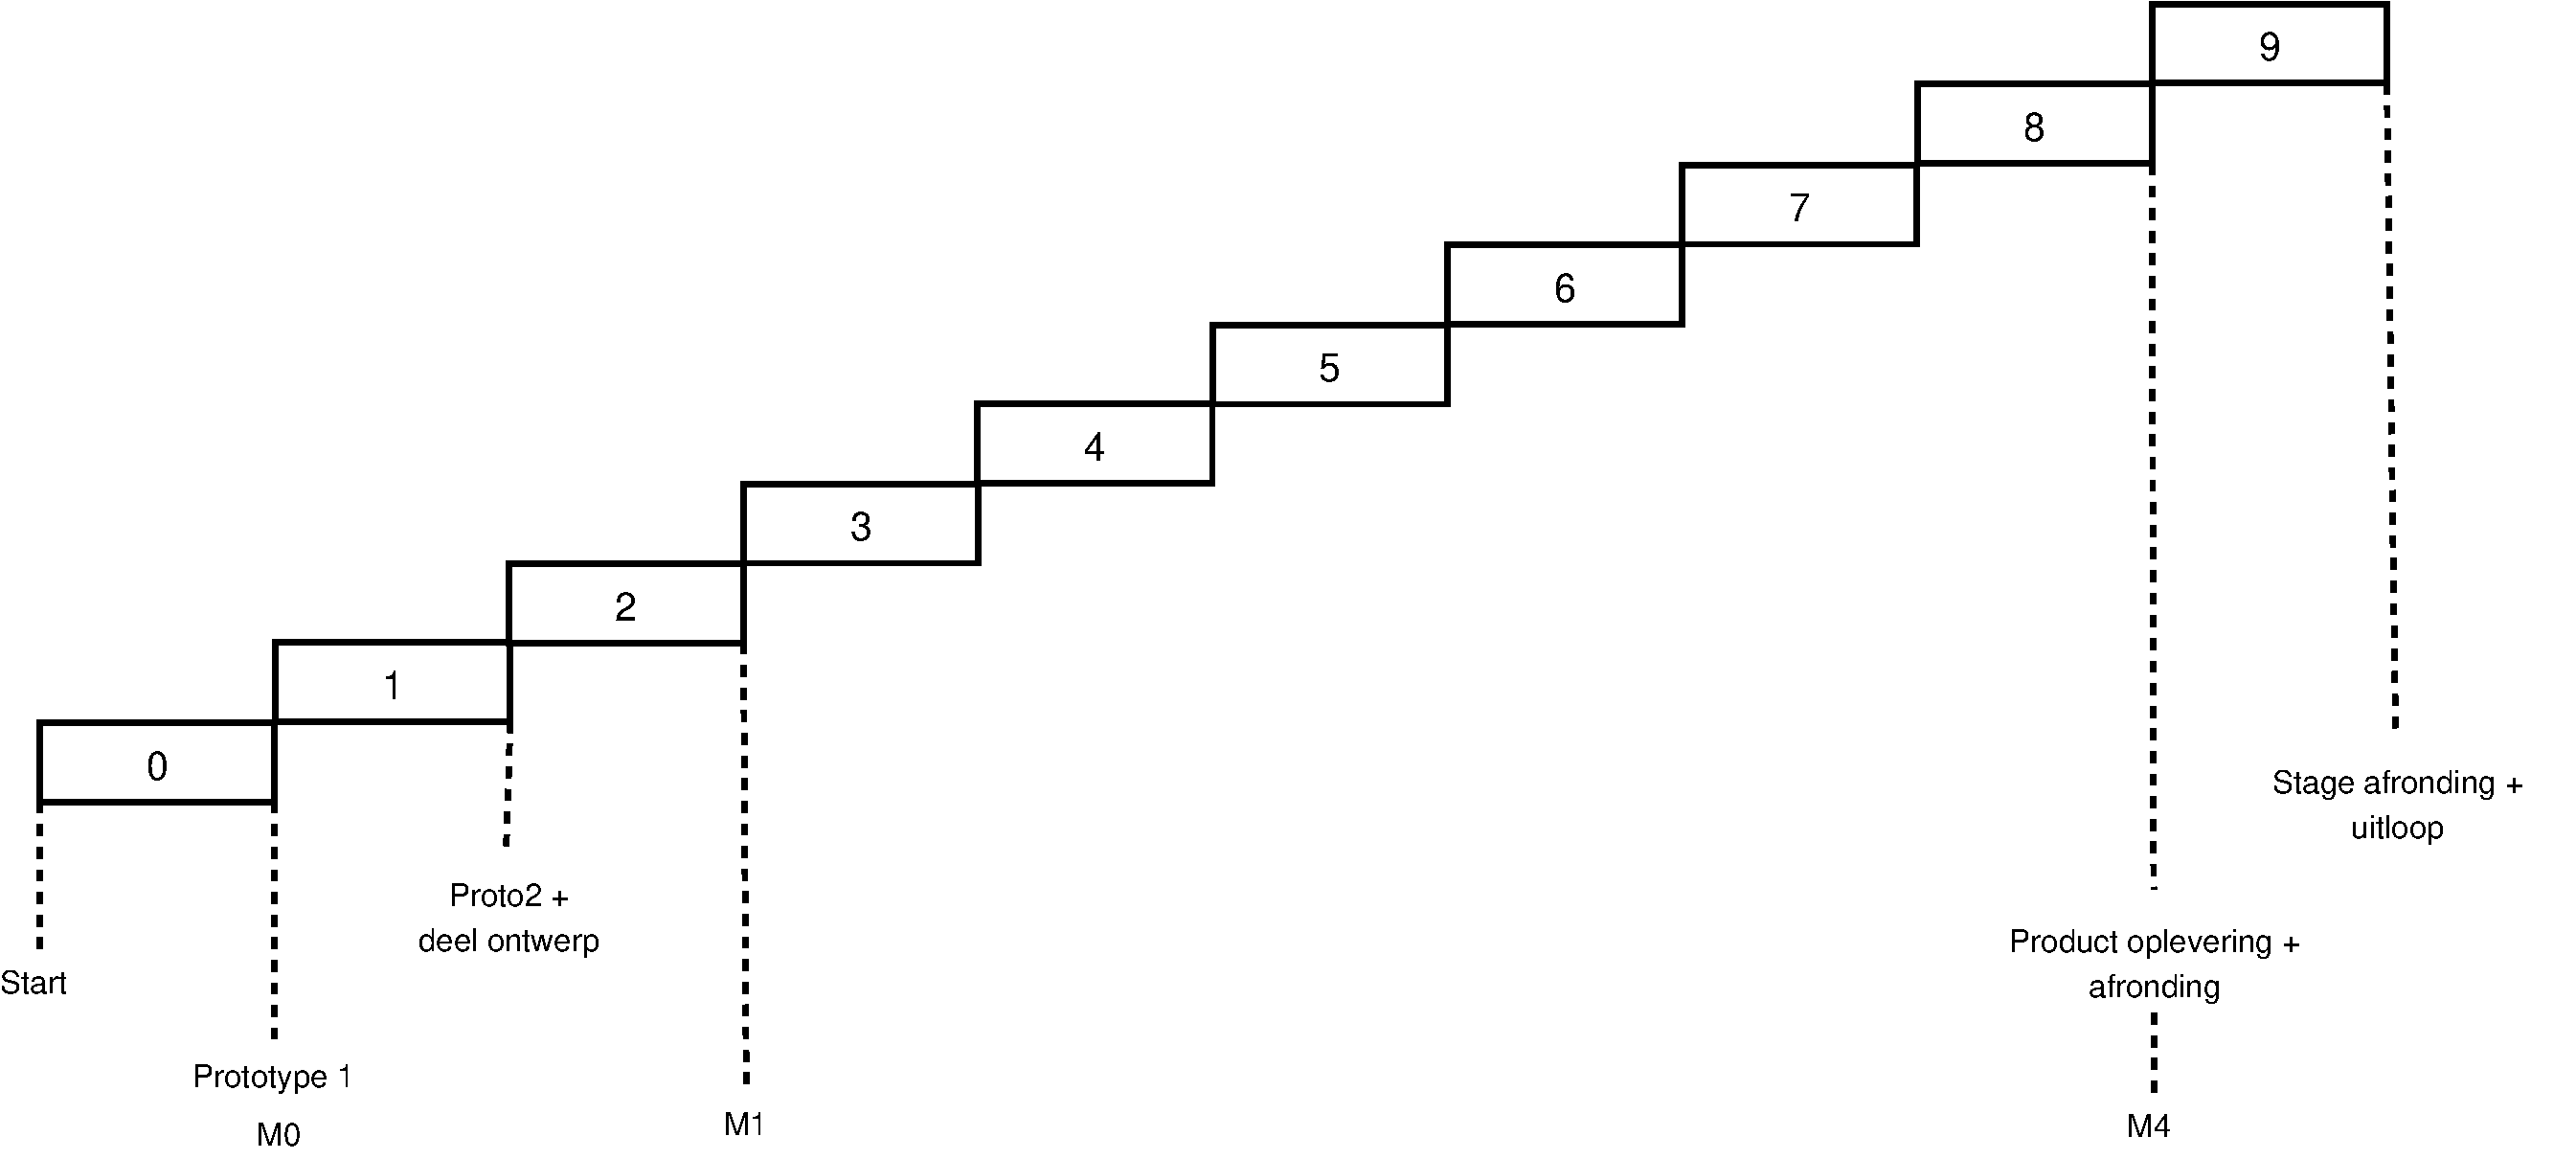
\includegraphics[width=20cm]{planning}
\end{figure}

In dit schema geven de rechthoekige genummerde vakken de increments aan. De gestippelde lijnen geven de gepland afgeronde activiteiten aan en de geplande milestones.

\end{landscape}

\newpage
\subsection{Toelichting}
\index{Planning,toelichting}
\label{planning}

Zoals in de fasering op bladzijde \pageref{fasering} besproken werd, wordt het project ingedeeld in \index{Milestones}milestones. Deze zijn zelf weer opgedeeld in \'e\'en of meerdere \index{Increments}increments.

\begin{tabularx}{\textwidth}{|c|c|X|}
\hline
Increment&Datum&Activiteit\\
\hline
0&2 - 13 Februari&Opstellen en aanpassen Plan van Aanpak, analyses uitvoeren, prototype1\\
\hline
\multicolumn{3}{|l|}{\textbf{Milestone 0: Studie}}\\
\hline
%\hline
%\multicolumn{3}{|l|}{\textbf{Milestone 2: Ontwerp}}\\
%\hline
1&16 - 27 Februari&Prototype2 + deel ontwerp\\
2&1 - 12 Maart&\\
\hline
\multicolumn{3}{|l|}{\textbf{Milestone 1: Voorbereiding}}\\
\hline
3&15 - 26 Maart&\\
%\hline
%\multicolumn{3}{|l|}{\textbf{Milestone 3: Implementatie en testen}}\\
%\hline
4&29 Maart - 9 April&\\
5&12 - 23 April&\\
6&26 April - 7 Mei&\\
7&10 - 21 Mei&\\
8&24 Mei - 4 Juni&Afronden en opleveren product\\
\hline
\multicolumn{3}{|l|}{\textbf{Milestone 4: Product test release}}\\
\hline
9&7 - 18 Juni&Stage afronden, presentatie houden, stageverslag maken\\
\hline
\end{tabularx}

Zoals tijdens de probleemstelling (zie pagina \pageref{probleemstelling}) te zien is, zal al lopende het project extra functionaliteit aangedragen worden. Deze planning zal dan ook aangepast worden.

Het faseringsoverzicht op pagina \pageref{faseringoverzicht} laat zien dat de milestones door elkaar heen lopen. Daarom zijn milestone 2: ontwerp en milestone 3: implementatie en testen niet in deze planning opgenomen.

Tenslotte wil Delem dat ik maximaal \'e\'en dag in de week reserveer voor zaken die niet direct in verband staan met de HSB Bus Analyser, maar waar ik bijvoorbeeld Solutions werk ga doen. Dit omdat er tijdens het werken in een bedrijfssituatie regelmatig iets tussendoor komt wat hogere prioriteit heeft.
